The following version of \textit{parallel ripple search} (PRS) is slightly modified from the one proposed by Bidarra et al. \cite{PRS}.
At a high level, the algorithm avoids the shortcomings of the parallel approaches discussed above by dividing the search space evenly across threads and removing dependency on a shared structure of open vertices.

This is done by isolating individual searches to a subsection of the graph and then reconstructing the solution in a divide-and-conquer fashion.

\mypar{Overview} 
At its core,  PRS can be broken down into four distinct phases which will be referred to as: high-level graph generation, space flooding, path refinement, and reconstruction. 
This implementation splits the work between a \textit{coordinator thread} and \textit{search threads}.
The coordinator is a separate thread which guides and schedules the work done by the search threads.
The coordinator also facilitates messages passed, thus removing intra-search-thread communication outside of synchronizing on shared memory.
A diagram depicting the flow of data between the coordinator and each search thread can be found in \figref{fig:high_level_flow}.
The decision was made to use a fringe search for each individual search thread in this implementation. However, different searches could be used, which would also affect the overall quality and performance of the algorithm.

\begin{figure}[H]
    \centering
    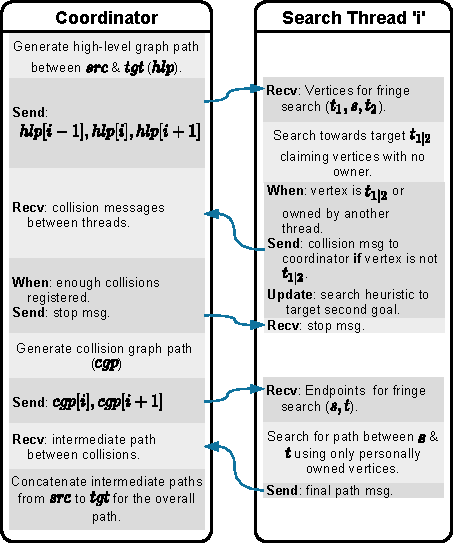
\includegraphics[width=.75\linewidth]{img/prs-flow-2.pdf}
    \caption{High-level logic and flow between the coordinator and search threads from PRS implementation.}
    \label{fig:high_level_flow}
\end{figure}

\mypar{High-Level Graph Generation}
The high-level graph is a coarse representation of the underlying search space and is used further to approximate where individual search threads should start from.
The high-level graph generation is an essential step in order to have distributed work amongst processes. 
A good high-level graph approximates the entire search space while reflecting expected vertex adjacencies. 
However, it should also be small, with a path length from source to target approximately equal to the number of available search threads.
Constructing a good high-level graph is a difficult task. However, this luckily only needs to happen once per graph. 
Therefore, once a high-level graph is generated, it can be stored and reused for subsequent path searches.
In this project, pathfinding was kept general enough to be applicable to any graph with vertex position information, making high-level graph generation more difficult. An applied use of PRS, where underlying graph characteristics are known a priori, could easily optimize this step. 
Further discussion on the details of the high-level graph generation and subsequently, the high-level path, will be deferred until \secref{sec:implementation}.

\begin{figure}[H]
    \centering
    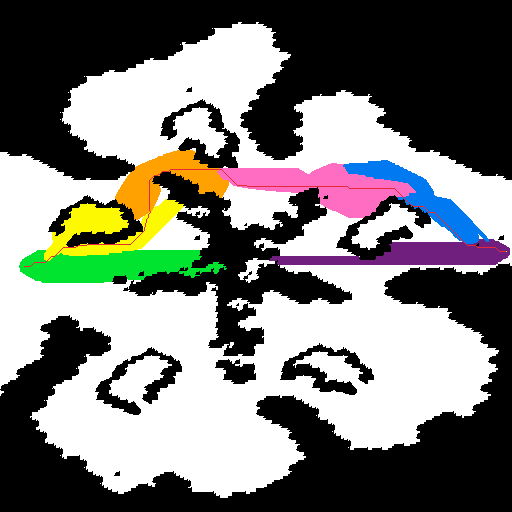
\includegraphics[width=.5\linewidth]{img/ripple.png}
    \caption{Final colored graph cache of PRS with 6 search threads with reconstructed path traced in red.}
    \label{fig:ripple_example}
\end{figure}

\mypar{Space Flooding} \label{par:space-flooding} 
In this initial search phase, a search thread $tid_i$ is started from each vertex of the high-level path, given two search targets, the source node of $tid_{i - 1}$ and $tid_{i + 1}$. 
These threads use a fringe search to explore the space around them, claiming vertices in cache as they are traversed, continuing until they reach the search space of a nearby thread or the current search target. 
After such a collision, the threads will change heuristic and start searching in the opposite direction, similar to bidirectional search. 
Two special cases are the search threads started from the global source and target vertices, which only have one neighboring thread, and thus will not perform a bidirectional search. During the exploration of the search space, the search threads communicate with the coordinator thread by informing it of encountered collisions between thread spaces. The coordinator thread registers the location and thread IDs of a collision and continuously tries to create a path via collision points from the source to target of the overall search. When such a path is found, the coordinator will halt the space flooding. An example of how threads flood the space can be seen in \figref{fig:ripple_example}.

\mypar{Path Refinement} 
After the threads have flooded the space and a path from the source to target has been found, each search thread will use a fringe search to find the shortest path between two collision points using only their region of claimed vertices. Under the assumption that the collision points between search threads lie close to an optimal path, restricting the search space of a thread in this manner will improve performance and have few adverse effects on the quality of the resulting path.

\mypar{Reconstruction} 
Once a path between each collision point is found, a path between the global source and target vertices can be reconstructed. 
The coordinator thread will simply concatenate the intermediate paths returned by each search thread in the order of the collision path.
